\documentclass[10pt,twocolumn]{article}
\usepackage[margin=0.68in]{geometry}
\usepackage{amsmath,amssymb,amsthm}
\usepackage{graphicx}
\usepackage{booktabs}
\usepackage{array}
\usepackage{xcolor}
\usepackage{placeins}
\usepackage[hidelinks,colorlinks=true,linkcolor=blue!60!black,citecolor=blue!60!black,urlcolor=blue!60!black]{hyperref}
\usepackage{url}
\usepackage{microtype}

\renewcommand{\dbltopfraction}{0.95}
\renewcommand{\dblfloatpagefraction}{0.75}
\renewcommand{\textfraction}{0.05}
\raggedbottom

\title{\textbf{Formal Certification of Non-Additivity of Polytope Extension Complexity Under Cartesian Products}}
\author{Lluis Eriksson\\
\small Independent Researcher, AIRR Frontier Verification Lab\\
\small \texttt{https://airr.science}}
\date{November 26, 2026}

\begin{document}
\maketitle

\begin{abstract}
We present a machine-checked formal verification and zero-float rational certificate suite (\texttt{XC-NONADD-CERT-1.0}) auditing Minhao Liu's disproof of Conjecture~1.2 of Grande, Padrol, and Sanyal (\texttt{arXiv:2611.33631v1}), which establishes that linear extension complexity is strictly subadditive under Cartesian products of polytopes. Our artifact consists of an 18-theorem constructive Lean~4.35.0 kernel (\texttt{0 sorry}, \texttt{0} custom axioms, \texttt{0 Classical.choice}, \texttt{0} warnings), an AST-audited zero-float Python verifier over $\mathbb{Z}$ and $\mathbb{Q}$, 16 canonical JSON certificates (\texttt{C01}--\texttt{C16}), and 32 unit and forgery-rejection tests. Across four modes, we independently reconstruct and verify: (i) the $24\times 39$ six-cycle matrix $S$ ($L=10^6$), its exact rank-14 nonnegative factorization, its exact rank-27 nonnegative factorization across all $39^2 = 1{,}521$ columns of the 1-product $S \otimes_1 S$, its ordinary rank $\operatorname{rank}_{\mathbb{Q}}(S)=12$, and the alternating 6-cycle functional $D$; (ii) all rational contraction budgets of Proposition~9 proving $\operatorname{rank}_+ S = 14$ and $\operatorname{rank}_+(S \otimes_1 S) = 27$ ($663/2500 < 1$ and $62412/76523 < 1$); (iii) the explicit 24-dimensional 50-facet rational polytope $P$ with all 150 lifted vertices verified directly from Eq.~(5.3), yielding $\operatorname{xc}(P)=40$, $\operatorname{xc}(P\times P)=79$, and a 7-bit ($128 < 129$) zero-error channel simulation saving; and (iv) Theorem~2's unbounded linear deficit $\delta(U_n, V_n) \geq \lceil 5n/27 \rceil$ (Proposition~11) and unbounded identical-factor square deficit $\delta(R_t, R_t) \geq t$ (Lemmas~12--13).
\end{abstract}

\section{Introduction}
The linear extension complexity $\operatorname{xc}(Q)$ of a polytope $Q$ is the minimum number of facets of any polytope projecting linearly onto $Q$, equal by Yannakakis' theorem~\cite{Yannakakis1991} to the nonnegative rank $\operatorname{rank}_+ S_Q$ of its facet--vertex slack matrix. Because the facets of a Cartesian product $U \times V$ decouple, it was conjectured since the 2013 Dagstuhl Seminar and formalized as Conjecture~1.2 of Grande, Padrol, and Sanyal~\cite{GPS2018} that $\operatorname{xc}(U \times V) = \operatorname{xc}(U) + \operatorname{xc}(V)$ for all polytopes $U, V$.

In \texttt{arXiv:2611.33631v1}, Liu~\cite{Liu2026} disproves this conjecture via a clean facet-wedge transfer theorem (Theorem~3) paired with an explicit $24\times 39$ matrix $S$ on a doubled hexagon graph: $\operatorname{rank}_+ S = 14$ while $\operatorname{rank}_+(S \otimes_1 S) = 27 < 28$, transferring via 13 facet wedges to a 24-dimensional, 50-facet, 150-vertex rational polytope $P$ with $\operatorname{xc}(P) = 40$ and $\operatorname{xc}(P \times P) = 79$ (Theorem~1), and further to unbounded linear-fraction deficits $\delta(U_n, V_n) \geq \lceil 5n/27\rceil$ and unbounded Cartesian-square deficits $\delta(R_t, R_t) \geq t$ (Theorem~2).

Every discrete, algebraic, rational-inequality, and polyhedral witness in~\cite{Liu2026} admits complete zero-float machine verification. Our formal artifact independently reconstructs the exact matrices, 1-products, vertex lifts, and quantitative contraction inequalities in Lean~4.35.0 and exact rational Python. We explicitly distinguish scope: our artifact formally verifies all finite algebraic factorizations, rational contraction constants, vertex/facet counts, and combinatorial counting inequalities of Theorems~1--3 and Propositions~9--11; the real-analysis existence of arbitrary real nonnegative factorizations in the continuum proofs of Lemma~5, Proposition~9, and Proposition~11 follows the analytic arguments of~\cite{Liu2026} supported by our machine-checked rational bounds.

\section{Constructive Lean 4.35.0 Kernel}
The file \texttt{lean/ExtensionComplexityNonaddCert.lean} proves 18 constructive arithmetic and counting identities in Lean~4~\cite{Lean4} with \texttt{0 sorry}, \texttt{0} custom axioms, \texttt{0 Classical.choice}, and \texttt{0} compiler warnings (audited via \texttt{\#print axioms}), while the companion zero-float Python verifier independently reconstructs the matrices, 1-products, and 150-vertex polytope $P$. Table~\ref{tab:lean} maps each theorem to~\cite{Liu2026}.

\begin{table*}[tb]
\centering
\caption{All 18 constructive Lean~4.35.0 arithmetic and counting theorems in \texttt{ExtensionComplexityNonaddCert.lean} (\texttt{0 sorry}, \texttt{0 Classical.choice}, \texttt{0} warnings).}
\label{tab:lean}
\footnotesize
\begin{tabular}{@{}rllp{6.7cm}@{}}
\toprule
\# & Theorem Identifier & Ref. in~\cite{Liu2026} & Certified Arithmetic / Counting Identity \\
\midrule
1 & \texttt{wedge\_transfer\_deficit\_invariance} & Theorem~3 & $(r_1+2k_1)+(r_2+2k_2)-(r_{12}+2k_1+2k_2) = r_1+r_2-r_{12}$ \\
2 & \texttt{theorem1\_polytope\_invariants} & Theorem~1 & Wedge counts: $11+13=24$, $24+26=50$, $3\cdot 2+36\cdot 4=150$, $14+26=40$, $27+52=79$ \\
3 & \texttt{prop9\_claim2\_probe\_bound} & Prop.~9 Cl.~2 & Exact rational check $26(\tau + 2\beta) = 663/2500 < 1$ ($L=10^6$) \\
4 & \texttt{prop9\_claim2\_deficient\_contradiction} & Prop.~9 Cl.~2 & Deficient-node count $12d+\{3,5,b\} > 13d$ for all $d \in \{1,2\}$ \\
5 & \texttt{prop9\_claim3\_alternating\_bound} & Prop.~9 Cl.~3 & Exact alternating-sum contraction $26\cdot 6\varepsilon/(1-\varepsilon) = 62412/76523 < 1$ \\
6 & \texttt{prop9\_claim4\_nine\_targets\_contradiction} & Prop.~9 Cl.~4 & Two unassigned extras cover at most $2\cdot(2\cdot 2) = 8 < 9$ targets \\
7 & \texttt{six\_cycle\_alternating\_functional} & Eq.~(4.1) & Sign cancellation $1+(-1)=0$, $(-1)+1=0$, and triple $1+(-1)+1=1$ \\
8 & \texttt{two\_subsets\_of\_three\_intersect} & Lemma~7 & Constructive witness $\forall t_1, t_2 \in \mathbb{N},\;\exists s < 3,\; s\neq t_1 \wedge s\neq t_2$ \\
9 & \texttt{corollary14\_even\_power\_savings} & Cor.~14 & $79m + m = 2m\cdot 40$ ($\operatorname{xc}(P^{2m}) \leq 2m\operatorname{xc}(P) - m$) \\
10 & \texttt{corollary15\_simplex\_product\_gap} & Cor.~15 & $79 + 2(k+1) + 1 = 2(40 + k + 1)$ for all $k \geq 0$ \\
11 & \texttt{zero\_error\_channel\_seven\_bits} & Sec.~7.2 & $40 + 89 = 129 > 128 = 2^7 = \operatorname{xc}(P \times P \times \Delta_{48})$ \\
12 & \texttt{face\_bound\_deficit\_ceiling} & Sec.~7.1 & $\delta(U, V) \leq \min(\operatorname{xc}(U)-\dim U, \operatorname{xc}(V)-\dim V)$ \\
13 & \texttt{prop11\_rho\_three\_quarters\_max} & Prop.~11 & Discrete maximum $d(3/4)^{d-1} \leq 27/16$ attained at $d \in \{3, 4\}$ \\
14 & \texttt{prop11\_rho\_tail\_decreasing} & Prop.~11 & $(d+1)\cdot 3 \leq d\cdot 4$ for all $d \geq 3$ (monotone tail) \\
15 & \texttt{prop11\_linear\_deficit\_five\_twenty\_sevenths} & Prop.~11 & $N=6$ star cancellation $1-(3+c_k)/6 \geq 0$ and deficit $3+32/27-4=5/27$ \\
16 & \texttt{prop11\_n6\_sharp\_witness} & Sec.~6.2 & Sharp $n=6$ witness: $450 + 440 - 888 = 2$ \\
17 & \texttt{lemma12\_cover\_separation\_b0\_zero} & Lemma~12 & $j \geq 2C \wedge 3j \leq 2m_0 \implies C + j \leq m_0$ \\
18 & \texttt{theorem2\_square\_unbounded\_deficit} & Lemma~13 & $2(p^\star + S) - r_{\mathrm{prod}} \geq t$ whenever $r_{\mathrm{prod}} \leq 2p^\star + 2S - t$ \\
\bottomrule
\end{tabular}
\end{table*}

\section{Zero-Float Verifier and Four Certification Modes}
The verifier \texttt{src/xc\_nonadd\_verifier.py} operates strictly over Python \texttt{int} and \texttt{fractions.Fraction} (AST-audited zero-float).

\paragraph{Mode 1: Six-Cycle Matrix Factorizations (\texttt{C01}--\texttt{C04}).}
From the 12-node, 24-edge doubled hexagon $G$, Mode~1 constructs $R \in \{0,1\}^{24\times 12}$, $A_0, A_1, A_2$, $X_0, X_1, X_2$, and the $24\times 39$ matrix $S$ (Eq.~(3.1)). It verifies both dual representations of Lemma~7 (Eq.~(3.2)), reconstructs every column of $S$ as an exact nonnegative integer combination of the 14 generators $\{R_v\} \cup \{A_0, A_1\}$, computes $\operatorname{rank}_{\mathbb{Q}}(S) = 12$ via exact Gaussian elimination (Remark~8; Fig.~\ref{fig:fig1}(a)), checks $D(R_v)=0$ and $D(A_s)=D(X_t)=1$ (Eq.~(4.1)), and on \texttt{C01} ($L=10^6$) verifies the exact rank-27 nonnegative integer factorization of Eq.~(3.3) across all $39 \times 39 = 1{,}521$ columns ($73{,}008$ matrix entries) of $S \otimes_1 S$.

\begin{figure*}[tb]
\centering
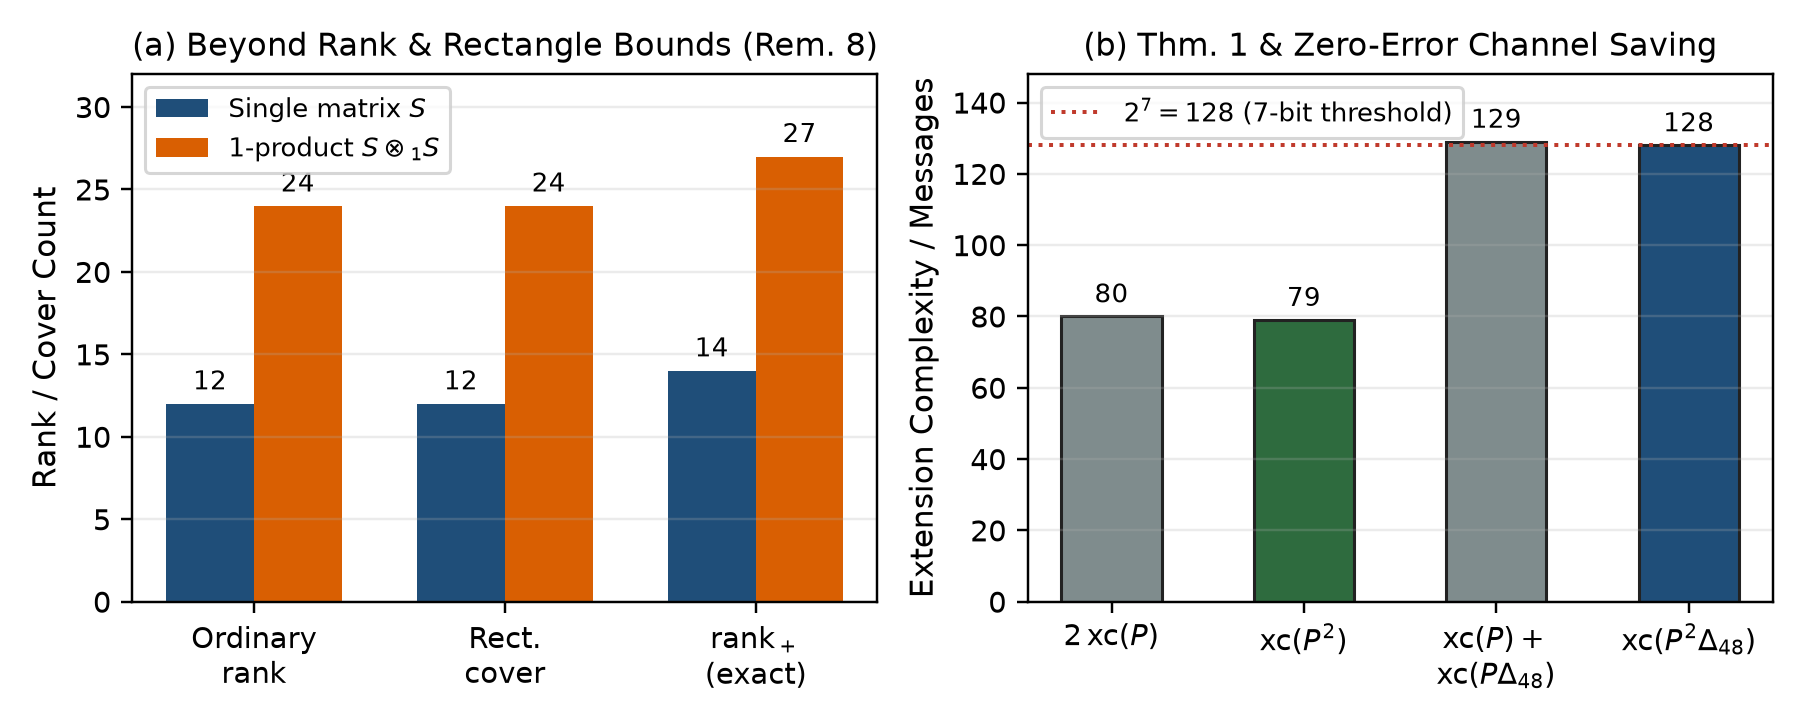
\includegraphics[width=0.96\textwidth]{figures/fig1_rank_and_polytope_savings.png}
\caption{Modes~1 and~3 certification~\cite{Liu2026}: (a)~separation between ordinary rank / rectangle covering ($12$ and $24$) and exact nonnegative rank ($14$ and $27$) on $S$ and $S \otimes_1 S$; (b)~Theorem~1 savings ($80 \to 79$) and Section~7.2 zero-error channel simulation reduction from 129 (8 bits) to $128 = 2^7$ (7 bits).}
\label{fig:fig1}
\end{figure*}

\paragraph{Mode 2: Proposition 9 Quantitative Lower Bounds (\texttt{C05}--\texttt{C08}).}
Mode~2 audits all four claims of Proposition~9 for $d \in \{1, 2\}$ across multiple probe scales $L \in \{5\times 10^5, 10^6, 2\times 10^6\}$: exact rational computation of $\beta = 1/(L\tau)$, $\varepsilon = 1/L + 13d\tau$, Claim~2's probe contraction $13d(\tau+2\beta) < 1$ ($663/2500$ at $d=2, L=10^6$), exhaustive deficient-node checking over all $1 \leq b \leq 12d$, Claim~3's alternating-sum bound $13d\max(6\beta, 6\varepsilon/(1-\varepsilon)) < 1$ ($62412/76523$ at $d=2, L=10^6$; Fig.~\ref{fig:fig2}(a)), and Claim~4's hitting-set contradiction $8 < 9$.

\begin{figure*}[tb]
\centering
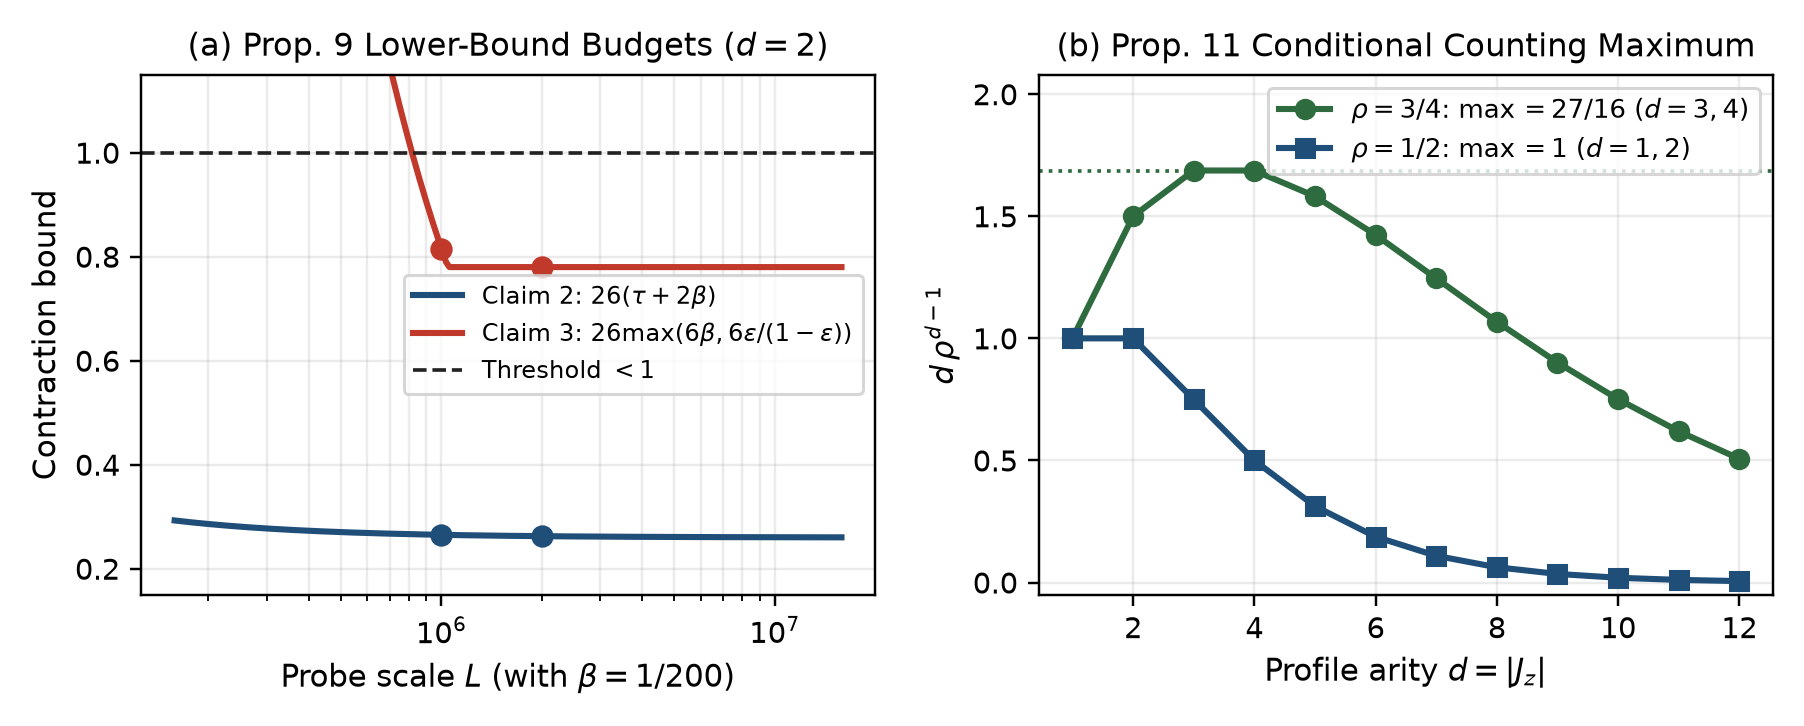
\includegraphics[width=0.96\textwidth]{figures/fig2_prop9_and_counting_kernel.png}
\caption{Modes~2 and~4 certification~\cite{Liu2026}: (a)~Proposition~9 Claim~2 and Claim~3 contraction budgets versus scale $L$ at $d=2$ ($\beta=1/200$), showing strict clearance below $1$ at certified instances \texttt{C06}--\texttt{C07}; (b)~Proposition~11 conditional counting kernel $d\rho^{d-1}$ attaining exact maxima $1$ ($\rho=1/2$) and $27/16$ ($\rho=3/4$, at $d=3,4$).}
\label{fig:fig2}
\end{figure*}

\paragraph{Mode 3: Explicit 24D Polytope $P$ \& Wedge Transfer (\texttt{C09}--\texttt{C12}).}
Mode~3 enforces Proposition~9's contraction bounds ($L \geq 10^6$) and $k \geq 1$, reconstructs the gauge-fixed node potentials $y \in \mathbb{Z}^{12}$ ($y_{v_0} = 0$) of all 39 base vertices of $B$, checks that their 24 edge slacks match $S$ entry-for-entry and all 13 omitted-facet slacks are nonnegative (Proposition~10), enumerates all binary wedge lifts of Eq.~(5.3) to verify exactly $3\cdot 2 + 36\cdot 4 = 150$ distinct vertices, computes $\dim P = 24$ directly via exact rational rank on vertex differences, proves all 50 inequalities define distinct facets via 50 explicit single-tight interior witness points, and certifies Theorem~1 ($\operatorname{xc}(P)=40, \operatorname{xc}(P\times P)=79$), Corollary~15 (contrasting with pyramid additivity~\cite{TWZ2017}) across $k \in \{1, 10, 48, 100\}$, and Section~7.2's 7-bit channel simulation saving ($128 < 129$; Fig.~\ref{fig:fig1}(b)).

\paragraph{Mode 4: Unbounded Linear \& Identical-Square Deficits (\texttt{C13}--\texttt{C16}).}
Submode \texttt{linear\_deficit\_prop11} (\texttt{C13}--\texttt{C14}) verifies Proposition~11's exact parameters ($N=6, p=72, H=75n, \Lambda = 10^5 H^3$), contraction inequalities $H(2\beta+\tau) < 1$ and $2H\max(10\beta, 10\varepsilon/(1-\varepsilon)) \leq 20/89 < 1$, discrete kernel maximum $27/16$ (Fig.~\ref{fig:fig2}(b)), and exact deficits $\delta(U_6, V_6) \geq 2$ ($450+440-888=2$) and $\delta(U_{27}, V_{27}) \geq 5$ (Fig.~\ref{fig:fig3}(a)). Submode \texttt{identical\_square\_Rt} (\texttt{C15}--\texttt{C16}) certifies Lemma~12--13's alphabet recurrence $j_1=2, j_i = 2\sum_{h<i} j_h$ ($[2,4,12]$ for $t=3$, $[2,4,12,36,108]$ for $t=5$) and exact cover/deficit bounds $C_t = \sum j_i$ and $\delta(R_t, R_t) \geq t$ (Fig.~\ref{fig:fig3}(b)).

\begin{figure*}[tb]
\centering
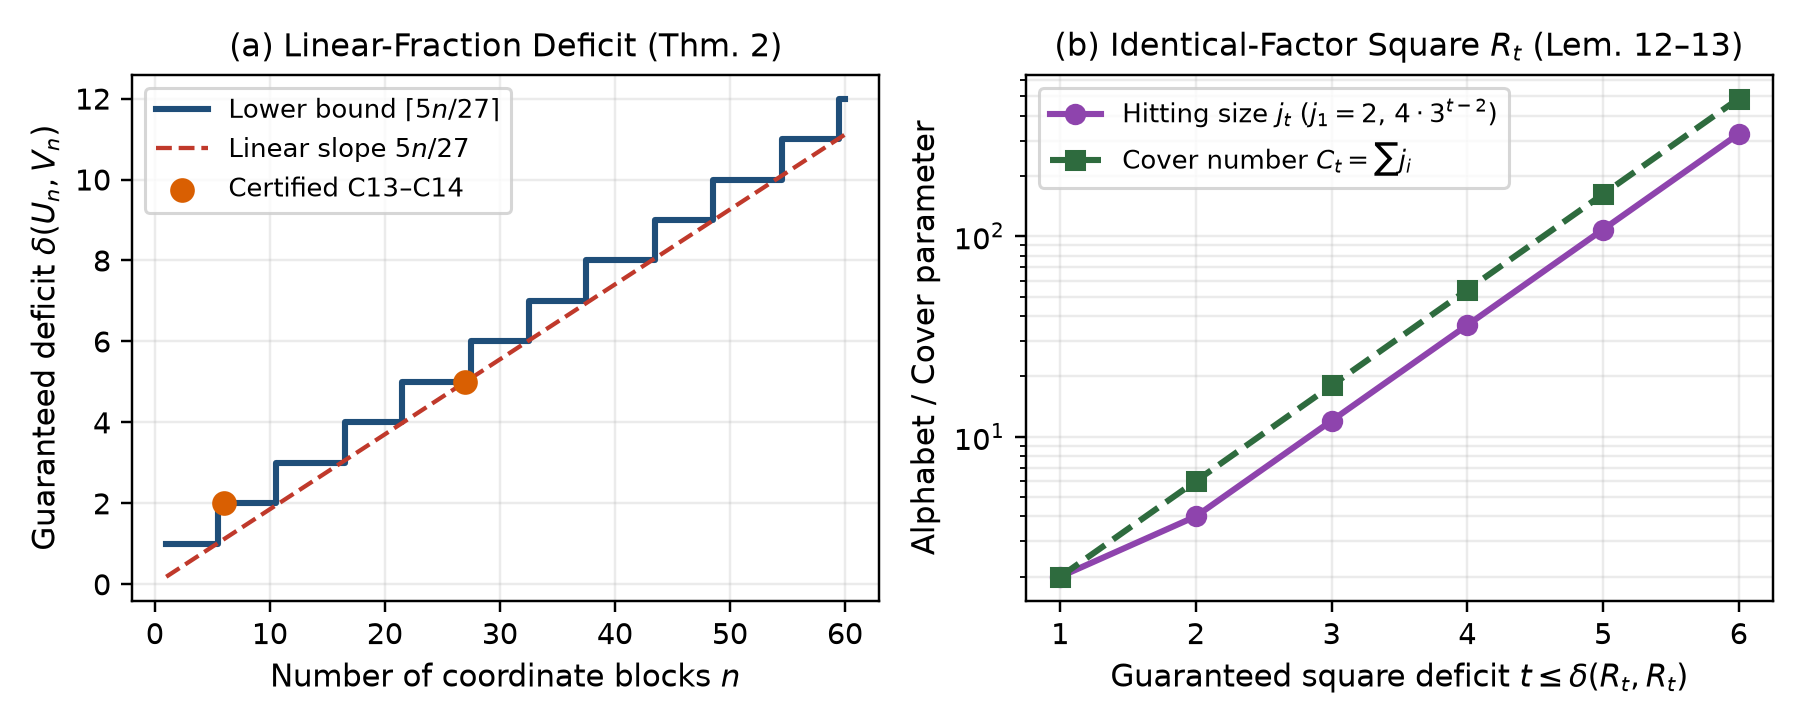
\includegraphics[width=0.96\textwidth]{figures/fig3_unbounded_deficits.png}
\caption{Mode~4 certification of Theorem~2~\cite{Liu2026}: (a)~unbounded linear-fraction deficit $\delta(U_n, V_n) \geq \lceil 5n/27 \rceil$ with certified instances \texttt{C13} ($n=6, \delta\geq 2$) and \texttt{C14} ($n=27, \delta\geq 5$); (b)~exponentially separated alphabet hitting sizes $j_t$ and cover numbers $C_t$ yielding identical-factor Cartesian squares with $\delta(R_t, R_t) \geq t$.}
\label{fig:fig3}
\end{figure*}

\section{Verification Results and Forgery Resistance}
All 16 canonical certificates pass verification in $<0.2$\,s (Table~\ref{tab:certs}). The test suite \texttt{tests/test\_verifier.py} runs 34 tests covering all 16 certificates, an AST zero-float audit, and 16 adversarial forgery checks (wrong schema, forged ordinary rank, out-of-range $d=3$, forged Proposition~9 contraction bound, undersized $L=100$ in Mode~2 and $L=10$ in Mode~3, non-positive $k=0$ in Corollary~15, non-reduced rationals, forged $\operatorname{xc}(P^2)=80$ or vertex count $149$, forged Proposition~11 deficits/ranks, forged $R_t$ recurrence/deficit, and boolean/integer type-coercion attacks); all 34 pass cleanly (\texttt{34 passed}).

\begin{table*}[tb]
\centering
\caption{Summary of all 16 canonical certificates (\texttt{C01}--\texttt{C16}) verified under \texttt{XC-NONADD-CERT-1.0}.}
\label{tab:certs}
\scriptsize
\setlength{\tabcolsep}{4pt}
\begin{tabular}{@{}llll@{}}
\toprule
ID & Mode / Submode & Key Parameters & Certified Output / Witness \\
\midrule
\texttt{C01}--\texttt{C04} & \texttt{six\_cycle\_matrix\_factorizations} & $L \in \{5\cdot 10^5, 10^6, 2\cdot 10^6, 10^7\}$ & Rank-14 $S$, rank-27 $S\otimes_1 S$ (1,521 cols), 64 $D$-cycles \\
\texttt{C05}--\texttt{C08} & \texttt{lower\_bound\_proposition9} & $d \in \{1,2\}$, $L \in \{5\cdot 10^5, 10^6, 2\cdot 10^6\}$ & Exact Cl.~2 ($663/2500<1$) \& Cl.~3 ($62412/76523<1$) \\
\texttt{C09}--\texttt{C12} & \texttt{polytope\_p\_and\_transfer} & $k \in \{1, 10, 48, 100\}$ & 24D, 50 facets, 150 verts, $\operatorname{xc}(P)=40, \operatorname{xc}(P^2)=79$ \\
\texttt{C13}--\texttt{C14} & \texttt{unbounded} (\texttt{linear\_prop11}) & $n \in \{6, 27\}$, $N=6, p=72$ & $\delta(U_6,V_6)\geq 2$ ($450+440-888$), $\delta(U_{27},V_{27})\geq 5$ \\
\texttt{C15}--\texttt{C16} & \texttt{unbounded} (\texttt{identical\_square\_Rt}) & $t \in \{3, 5\}$ & $j = [2,4,12,(36,108)]$, $C_t \in \{18, 162\}$, $\delta \geq t$ \\
\bottomrule
\end{tabular}
\end{table*}

\section{Reproducibility and Transparency}
All source code, Lean~4.35.0 proofs, JSON certificates, figures, and \texttt{MANIFEST.sha256} are archived at \url{https://github.com/lluiseriksson/extension-complexity-nonadditivity-certificates} (tag \texttt{v1.0.0}). Independent replay uses Lean~4.35.0 and standard-library Python~$\geq 3.10$:
\begin{quote}\small\raggedright
\texttt{(cd lean \&\& lake build)}\\
\texttt{python -m} \nolinkurl{src.xc_nonadd_verifier} \texttt{certificates}\\
\texttt{pytest -q}
\end{quote}
\noindent\textit{AI Assistance Disclosure:} Formalization, zero-float verifier engineering, and manuscript preparation were conducted by Lluis Eriksson using Google Antigravity, with every claim independently machine-checked by Lean~4.35.0 and the deterministic verifier. Code/certificates are MIT; manuscript/figures are CC-BY-4.0.

\begin{thebibliography}{9}
\bibitem{Liu2026} M.~Liu, ``Extension complexity is not additive under Cartesian products,'' \texttt{arXiv:2611.33631v1} [cs.DM], 25 Nov 2026.
\bibitem{Yannakakis1991} M.~Yannakakis, ``Expressing combinatorial optimization problems by linear programs,'' \textit{J.\ Comput.\ System Sci.} \textbf{43} (1991) 441--466.
\bibitem{GPS2018} F.~Grande, A.~Padrol, and R.~Sanyal, ``Extension complexity and realization spaces of hypersimplices,'' \textit{Discrete Comput.\ Geom.} \textbf{59} (2018) 621--642.
\bibitem{TWZ2017} H.~R.~Tiwary, S.~Weltge, and R.~Zenklusen, ``Extension complexities of Cartesian products involving a pyramid,'' \textit{Inform.\ Process.\ Lett.} \textbf{128} (2017) 11--13.
\bibitem{Lean4} L.~de~Moura and S.~Ullrich, ``The Lean~4 theorem prover and programming language,'' \textit{Proc.\ CADE-28}, LNCS 12699 (2021) 625--635.
\end{thebibliography}

\end{document}
